\documentclass{article}
\usepackage{amsmath, amsthm, amssymb} % maths stuffs
\usepackage[english, main=greek]{babel} 
\usepackage[a4paper, total={6in, 10in}]{geometry}
\usepackage{graphicx}  % for images
\usepackage{subcaption} % for multiple images in the same figure
\usepackage{titling}


\setlength{\parindent}{0pt}
\setlength{\parskip}{5pt}

\title{Sup}
\date{}

\begin{document}
\maketitle

\section{oohh yeahhh}
Let's see how this works

\subsection{Ti simainei diakritiki ikanotita organou?}
Legetai i mikroteri dinati metavoli tis metroumenis posotitas pou mporei na ginei antilipti apo to organo.

\subsection{Ti einai i polwsi organou?}
Legetai i tasi tou organou na dinei diaforetiki endeiksi apo tin pragmatikh timh kata mia statheri posotita. Thetikh h arnhtikh.

\subsection{Se ti daiferei apo tin akriveia diasporas?}
Polwsi perigrafei poso proseggizei i endeiksi enos organou tin pragmatikh timh tou metroumenu megethous, i defteri perigrafei ti statistiki diaspora pou parousiazoun epanalamvanomenes metriseis tou organou.

\subsection{Pws orizetai i klasi enos organou?}
Einai i posotita $G=100*\frac{Dx}{xt}$, opou Dx megisto apolito sfalma, xt megisti endeiksi tou organou.

\subsection{Poia einai ta kiriotera eidi sfalmatwn?}
Xwrizontai se sistimatika kai tyxaia. Ta sistimatika xwrizontai kai se dinamika kai statika kai ofeilontai stin epidrasi tou perivallontos, stis diafores ateleies tou organou kai stis adinamies twn methodwn metrishs.

\subsection{Evaisthisia organou?}
O logos tis metavolis apokrishs pros ti metavoli tis diegershs.

\subsection{\emph{(Σεπ. 2013)} Ένας ηλεκτροκινητήρας για ορισμένες συνθήκες λειτουργίας απορροφά ηλεκτρική ισχύ $1KW$ και παράγει μηχανική ισχύ $0,9HP$. Αν η μηχανική ισχύ μετρήθηκε με μέγιστο σχετικό σφάλμα $2\%$ και η ηλεκτρική ισχύς με βαττόμετρο κλάσης $1\%$ και μέγιστης κλίμακας $1,5KW\%$ να υπολογιστεί το μέγιστο απόλυτο και σχετικό σφάλμα του βαθμού απόδοσης του κινητήρα.}

\emph{Παρόμοια με ασκ.3 Σελ. 40, Σελ. 25-6,33 για τύπους}

\section{Prostasia}
\subsection{Pote ginetai to revma epikindino? (Επικίνδυνα σε θέλω, μέσα μου κυλάαααααααας)}
Gia panw apo $100mA$ gia diarkeia rohs $1\;sec$ opou pathainoume kardiakh prosvolh. Oles oi taseis katw apo $50V$ thewrountai akindines.

\subsection{Poia einai ta apotelesmata ilektropliksias?}
Gia xamiloteres entaseis revmatwn, kardiaki prosvolh. Gia ipsiloteres, myuikh systolh, systolh tou myokardiou (kardiakh prosvolh), anapnefstiki paralysh, egkavmata.

\subsection{Apo posous paragontes epireazetai i antistasi tou anthrwpinou swmatos?}
Kiriws apo tin katastasi tou dermatos (mikroterh antistasi gia mikro derma).

\subsection{To sinexes h to enallassomeno revma einai pio epikindino gia ton anthrwpo?}
To enallassomeno pio epikindino, eidikotera stis xamiles sixnothtes.

\subsection{Ti einai geiwsi prostasias kai geiwsi leitourgias?}
O oudeteros komvos twn trifasikwn hlektrikwn diktywn legetai geiwsi leitourgeias. I geiwsi prostasias einai to ekswteriko metalliko perivlima mias siskevis.

\subsection{Ti einai amesi geiwsi kai ti oudeterwsi?}
H geiwsi prostasias ginetai eite me amesi geiwsi h oudeterwsi. Stin amesi geiwsi o agwgos prostasias ston pinaka dianomis sindeetai mesw xalkinou agwgou sto ilektrodio geiwshs pou einai vythismeno sto edafos.  O agwgos prostasias sindeetai me oles ti revmatolhpsies. Stin oudeterwsi o agwgos prostasias sindeetai ston pinaka dianomis me ton oudetero agwgo pou einai geiwmenos konta stin eisodo tis paroxis tou katanalwth.

\subsection{Ti legetai antistash geiwshs?}
Legetai h antistash diaxyshs se seira me thn antistash tou agwgou pou sindeei ton agwgo prostasias me to hlektrodio geiwshs. Oso mikroterh toso kaliterh geiwsh.

\subsection{Poios einai o skopos egkatastashs metasxhmatistwn apomonwshs?}
Aytoi oi M/T isxyws einai synhtws 1:1 me ageiwto deyterevwn. An ena stoixeio tash akoumphsei to metalliko perivlhma enos organou, tote den diatrexei kindyno kapoiow pou tha piasei to perivlhma tou organou, giati den mporei na kleisei kyklwma afou to defterevwn den einai geiwmeno kai den yparxei galvanikh syndesh prwtevontos me to defterevwn.

\subsection{Ti einai oi diakoptes diafyghs?}
Ena eidos prostasias apo thn hlektroplhksia. Yparxoun oi diakoptes diafyghs tashs kai entashs (diaforikoi). 

O \textbf{diakopths diafyghs tashs} periexei ena phnio tashs. Otan h tash ypervei ta 50V, elkei ton oplismo tou kai diakoptei oles tis faseis kai ton oudetero se dekata tou defteroleptou.
O \textbf{diakopths diafyghs entashs} periexei enan metasxhmatisth kai ena phnio diakophs/diafyghs. Otan den yparxei epafh metaksy stoixeioy me tash kai toy ekswterikou perivlhmatos, ta revmata twn agogwn trofodosias einai isa kai dimioyrgan antitheta polwmena magnhtika pedia ta opoia allhloejoydeterwnontai. Otan yparxei syndesh metaksy stoixeiwn kai perivlhmatos, epagetai tash sto defterevwn tou M/T, energopoieitai to phnio diafyghs kai diakoptetai to kyklwma se liga defterolepta.

\subsection{Pws prostatevontai ta kyklwmata? Pou pane ta mpalonia?}
Me asfaleies kai aftomatoys diakoptes. An h entash toy revmatos perasei ena orio, diakoptetai to kyklwma. Apofevgetai etsi h proklhsh pyrkagias logw vraxykyklwmatos kai h katastrofh twn agwgwn twn syskevwn.

\subsection{Arxh leitourgias aftomatwn diakoptwn}
Exoun ena thermiko kai ena magnhtiko stoixeio. 

To thermiko stoixeio einai ena dimetalliko elasma to opoio otan thermanthei kathws diareetai apo revma ligo perissotero apo to kanoniko, paramorfwnetai kai analamvanei thn diakoph tou kyklwmatos meta apo ligo. 

To magnhtiko stoixeio einai ena phnio me pyrhna kai enan oplismo to opoio diegeiretai kai diakoptei aftomata to kyklwma otan to revma ginei poly megalo.

\subsection{Poio skopo eksyphretoun oi aftomatoi diakoptes gia elleipsh tashs kai poio oi aftomatoi gia diadoxh fasewn?}

Oi \textbf{aftomatoi diakoptes gia elleipsh tashs} diakoptoun to kyklwma otan h tash pesei katw apo mia sygkekrimenh timh (pretty self explanatory really). 

Oi \textbf{aftomatoi diakoptes gia diadoxh fasewn} diakoptoun to kyklwma an h trifasikh syndesmologia egine lathos kai h diadoxh twn fasewn einai antitheth apo thn provlepomenh. Efarmozontai gia prostasia hlektrokinhthrwn oi opoioi allazoun fora peristrofhs otan allazei h diadoxh twn fasewn.

\section{Ηλεκτρικός Θόρυβος}
\subsection{Τι λέγεται ηλεκτρικός θόρυβος?}
Λέγονται οι παρενοχλήσεις από ανεπιθύμητα σήματα στο κύκλωμα που μας ενδιαφέρει.

\subsection{Ποιές είναι οι κύριες πηγές ηλεκτρικού θορύβου?}
Ειναι ημιαγωγοί που χρησιμοποιούνται σαν διακόπτες, οι εκκενώσεις κάθε μορφής, οι ηλεκτροκολλήσεις, οι λάμπες φθορισμού και οι λυχνίες θύρατρον.

\subsection{Ποιά είναι τα είδη σύζευξης ηλεκτρικού θορύβου?}
\begin{itemize}
    \item Ηλεκτροστατική ή χωρητική σύζευξη
    \item Μαγνητική ή επαγωγική
    \item Ηλεκτρομαγνητική
    \item Σύζευξη κοινής αντίστασης
    \item O \foreignlanguage{english}{Merzbow} (ειναι αντι\foreignlanguage{english}{SOS} αυτό δεν πέφτει ποτέ)
\end{itemize}

\emph{Σελ. 56-7}
\subsection{Εξηγήστε τη φύση της ηλεκτροστατικής και της μαγνητικής \linebreak σύζευξης}
Λέγονται και οι δύο μικρής απόστασης σύζευξης γιατί εξανεμίζονται όταν η απόσταση μεταξύ πηγής και δέκτη του θορύβου είναι μεγάλη.

Η \textbf{ηλεκτροστατική σύζευξη} οφείλεται στην χωρητικότητα μεταξύ πομπού και δέκτη και ο θόρυβος λόγω της ηλεκτροστατικής σύζευξης αυξάνεται όταν:
\begin{itemize}
    \item Αυξάνεται η συχνότητα
    \item Aυξάνεται η αντίσταση εισόδου του οργάνου
    \item Αυξάνεται η χωρητικότητα μεταξύ πομπού και δέκτη του θορύβου
\end{itemize}

Η \textbf{μαγνητική σύζευξη} οφείλεται στην τάση αλληλεπαγωγής μεταξύ πηγής και δέκτη, δηλαδή στις τάσεις που δημιορυγούνται από επαγωγή λόγω μεταβολής μαγνητικών πεδίων. Ο θόρυβος αυξάνεται όταν:
\begin{itemize}
    \item Aυξάνεται η ένταση του μαγνητικού πεδίου
    \item Αυξάνεται ο εμπλεκόμενος με το μαγνητικό πεδίο βρόγχος του δέκτη
    \item Αυξάνεται η ταχύτητα μεταβολής του μαγνητικού πεδίου
    \item Μικραίνει η αντίσταση εισόδου
\end{itemize}
\emph{Σελ. 57-9}

\subsection{Εξηγήστε τη φύση της ηλεκτρομαγνητικής σύζευξης}
Η ηλεκτρομαγνητική ακτινοβολία που εκπέμπεται από ραδιοφωνικούς και τηλεοπτικούς πομπούς μπορεί να δημιουργήσει θόρυβο κυρίως σε πολύ λεπτές μετρήσεις, ακόμα και σε περιπτώσεις που ο πομπός βρίσκεται πολύ μακριά από τον δέκτη (σύζευξη θορύβου μεγάλης απόστασης).

\emph{Σελ. 60}

\subsection{Πότε εμφανίζεται σύζευξη κοινής αντίστασης?}
Εμφανίζεται όταν 2 ή και περισσότερα κυλώματα έχουν πολλούς κοινούς αγωγούς τροφοδοσίας και κατά συνέπεια τα ρεύματα των κυκλωμάτων περνούν από κοινές σύνθετες αντιστάσεις.

\emph{Σελ. 61}

\subsection{Να αναφερθούν τρόποι μείωσης του θορύβου}
\begin{itemize}
    \item Τοποθέτηση των διατάξεων μετρήσεων μακριά από τις πηγές θορύβου (ηλεκτροστατική, μαγνητική)
    \item Το "στρίψιμο" των καλωδίων στε ευαίσθητες μετρητικές διατάξεις (ηλεκτροστατική, μαγνητική)
    \item Χρήση φίλτρων τροφοδοσίας αν υπάρχει θόρυβος που προέρχεται από την τροφοδοσία. Είναι χαμηλοπερατά φίλτρα που αφήνουν να περάσει η συχνότητα τροφοδοσίας και απορρίπτουν τον θόρυβο (κοινής αντίστασης)
    \item Χρήση θωράκισης, δηλαδή κάλυψης ενός αγωγού/στοιχείου με κάλυμα με συγκεκριμένες ηλεκτρομαγνητικές ιδιότητες που αποτρέπουν λήψη και εκπομπή ηλεκτρικού θορύβου (αγώγιμα πλέγματα για ηλεκτροστατική, σιδηρομαγνητικό υλικό για μαγνητική, αγώγιμο υλικό/στρώματα αγώγιμου και σιδηρομαγνητικού υλικού για ηλεκτρομαγνητική)
    \item Χρήση σωστών γειώσεων (υποθέτω για κοινή αντίστασης, μαγνητική, ηλεκτροστατική)
    \item Χρήση αγωγών μικρής αντίστασης (κοινής αντίστασης)
    \item Αποφυγή κοινών συνδέσεων (κοινής αντίστασης) \foreignlanguage{english}{{(duh)}}
\end{itemize}
\emph{Σελ. 63-4}

\section{Μέτρηση ισχύος και ενέργειας}
\subsection{Να περιγράψετε την αρχή λειτουργίας αντισταθμισμένων βαττόμετρων}
Τα αντισταθμισμένα βαττόμετρα έχουν δύο πηνία τάσης, τα Π1 και Π2. Τα Π1 και Π2 είναι συνδεδεμένα σε σειρά μεταξύ τους και διαρρέονται με το ίδιο ρεύμα. Κατασκευαστικά, όμως, το Π2 είναι παράλληλα του πηνίου έντασης, αφαιρώντας το μαγνητικό πεδίο του Π2 από το πεδίο του πηνίου έντασης. Έτσι, στην ένδειξη του οργάνου δεν συμπεριλαμβάνεται η ισχύς που καταναλίσκεται στο πηνίο τάσης. Πρέπει όμως η σύνδεση του πηνίου τάσης να γίνει από την πλευρά της κατανάλωσης.

\emph{Σελ. 197-8}

\subsection{Να περιγράψετε τη μέτρηση ενεργού ισχύος με τη διάταξη \foreignlanguage{english}{Aron} σε τριφασικό σύστημα τριών αγωγών με συμμετρικές τάσεις}
\emph{Σελ. 202-3 πάνε διάβασε το από το βιβλίο και κουράγιο, μην πανικοβληθείς}

\subsection{Να περιγράψετε τη μέθοδο μέτρησης άεργου ισχύος σε τριφασικό σύστημα μετρήσεων με τρία βαττόμετρα}

\begin{figure}[h!]
    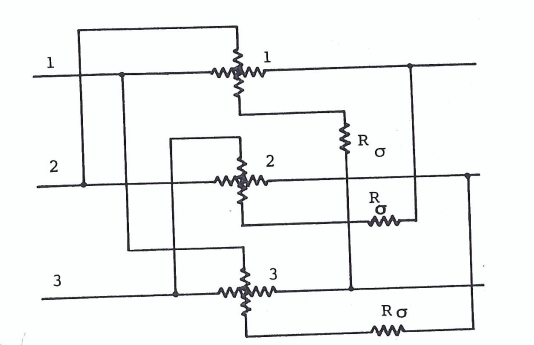
\includegraphics[width=\linewidth]{aei.png}
    \caption{Μετρητής άεργου ισχύος}
    \label{fig:4.3MAI}
\end{figure}

Η ένδειξη του βαττόμετρου 1 θα είναι: $U_{23}I_1\cos(90^\circ - \phi_1) = \sqrt{3}V_1I_1\sin(\phi_1) = \sqrt{3}Q_1$
\newpage

Οι ενδείξεις των 2 και 3 αντίστοιχα:

\begin{align*}
    U_{31}I_2\cos(90^\circ - \phi_2)=\sqrt3Q_2 \\
    U_{12}I_3\cos(90^\circ - \phi_3)=\sqrt3Q_3
\end{align*}

Η τριφασική άεργος ισχύς είναι ίση με με το άθροισμα των ενδείξεων των βαττομέτρων διαιρεμένο δια $\sqrt{3}$. Σε περίπτωση συμμετρικού φορτίου, αρκεί ένα από τα τρία βαττόμετρα. Η άεργη ισχύς σε αυτή την περίπτωση θα είναι η ένδειξη του βαττομέτρου επί $\sqrt{3}$.

\emph{Σελ. 205-6}
\subsection{Εξηγήστε πως μπορεί να μετρηθεί ο συντελεστής ισχύος συμμετρικού τριφασικού κυκλώματος με τη διάταξη \foreignlanguage{english}{Aron}.}
\emph{Σελ. 208 ντου δις λειτερ}

% MEROS B MEROS B MEROS B MEROS B MEROS B MEROS B MEROS B MEROS B MEROS B MEROS B MEROS B MEROS B MEROS B MEROS B MEROS B MEROS B MEROS B MEROS B MEROS B MEROS B MEROS B MEROS B MEROS B
% MEROS B MEROS B MEROS B MEROS B MEROS B MEROS B MEROS B MEROS B MEROS B MEROS B MEROS B MEROS B MEROS B MEROS B MEROS B MEROS B MEROS B MEROS B MEROS B MEROS B MEROS B MEROS B MEROS B
% MEROS B MEROS B MEROS B MEROS B MEROS B MEROS B MEROS B MEROS B MEROS B MEROS B MEROS B MEROS B MEROS B MEROS B MEROS B MEROS B MEROS B MEROS B MEROS B MEROS B MEROS B MEROS B MEROS B

\title{Μέρος Β}
%\date{}

\maketitle

\section{Εισαγωγή στα Συστήματα Μετρήσεων}
\subsection{Τι είναι μετατροπέας? Ποιοί είναι οι πιο διαδεδομένοι τύποι μετατροπών? Ποιά είναι η διαφορά μεταξύ ενός αισθητηρίου και ενός ανιχνευτή?}
Μετατροπέας λέγεται η διάταξη που απορροφά ενέργεια από ένα σύστημα και την μεταφέρει, αφού συνήθως τη μετατρέπει σε ενέργεια άλλης μορφής, ένα άλλο σύστημα.

Οι μετατροπείς που χρησιμοποιούνται για μετρήσεις είναι οι λεγόμενοι μετατροπείς εισόδου. Διεγείρονται από κάποια φυσική ποσότητα και δημιουργούν ένα σήμα εξόδου, συνήθως
ηλεκτρικό, το οποίο χρησιμοποιείται για την μέτρηση της αντίστοιχης φυσικής ποσότητας. Μετατροπείς εξόδου λέγονται οι μετατροπείς που μετατρέπουν ηλεκτρική ενέργεια 
σε ενέργεια άλλης μορφής, συνήθως μηχανική. Όταν χρησιμοποιούνται σε συστήματα ελέγχου λέγονται και ενεργοποιητές. Ένας μετατροπέας λέγεται ενεργός αν χρειάζεται 
για τη λειτουργία του μια εξωτερική πηγή ενέργειας. Ένας μετατροπέας λέγεται παθητικός αν δεν απατείται εξωτερική πηγή, αλλά η ενέργεια που απορροφάται από το μετρούμενο
σύστημα μετατρέπεται σε ενέργεια εξόδου (δηλαδή σε ενέργεια του σήματος που δημιουργείται σαν αποτέλεσμα του μετρούμενου μεγέθους). Οι πιο διαδεδομένοι τύποι μετατροπών 
είναι:

(Δεν ξέρω κατά πόσο αξίζει να μάθει κανείς αυτή τη λίστα τβη)

\begin{enumerate}
    \item Ηλεκτρομηχανικός τύπος 
    \item Τύπος ποτενσιόμετρου
    \item Τύπος διαφορικού μετασχηματιστή
    \item Τύπος πιεζοαντίστασης
    \item Φωτοηλεκτρικός τύπος
    \item Πιεζοηλεκτρικός τύπος 
    \item Θερμοηλεκτρικός τύπος
    \item Τύπος μεταβλητής ηλεκτρικής αντίστασης
    \item Τύπος θερμοδιαστολής
    \item Ηιμαγωγικοί μετατροπείς θερμοκρασίας
    \item Χωρητικός τύπος 
    \item Επαγωγικός τύπος
    \item Τύπος ταλαντωτή
    \item Τύπος \foreignlanguage{english}{Hall} και μανγητοαντίστασης
\end{enumerate}

\textbf{Αισθητήριο} λέγεται μια διάταξη που χρησιμοποιείται για την μέτρηση ή ανίχνευση ενός φυσικού μεγέθους ενώ \textbf{ανιχνευτής} είναι μια διάταξη που 
χρησιμοποιείται για την ανίχνευση ενός φυσικού μεγέθους.

\emph{Σελ. 271-3}
\subsection{Τι λέγεται ρύθμιση και τι ευαισθησία ενός συστήματος? Πότε λέμε ότι ένα σύστημα έχει γραμμικότητα μέτρησης και πότε ότι έχει γραμμική δυναμική συμπεριφορά?}
\scriptsize (Πήρε φόρα ο δικός σου)
\normalsize

\textbf{Ρύθμιση} ενός συστήματος μέτρησης λέγεται η διαδικασία κατά την οποία μεταβάλλεται αργά και με έναν γνωστό τρόπο η επιθυμητή είσοδος του συστήματος μέσα σε μια
περιοχή τιμών έτσι ώστε να καλυφθεί η περιοχή μέτρησης του συστήματος και να αντιστοιχηθεί σε κάθε τιμή της εξόδου μια τιμή της επιθυμητής εισόδου. Η γραμμική παράσταση
αυτής της αντιστοίχησης τιμών εισόδου και εξόδου λέγεται καμπύλη ρύθμισης.

\textbf{Ευαισθησία} λέγεται ο λόγος της μεταβολής της εξόδου προς τη μεταβολή της εισόδου στη μόνιμη κατάσταση λειτουργίας.

Ένα σύστημα έχει \textbf{γραμμικότητα μέτρησης} όταν η καμπύλη ρύθμισής του είναι μια ευθεία γραμμή.

Μπορεί ένα σύστημα να διέπεται από γραμμική διαφορική εξίσωση (\textbf{γραμμικότητα της δυναμικής του συστήματος}) αλλά να μην έχει γραμμικότητα μέτρησης.

\emph{Σελ. 292, 294}
\subsection{Τι γνωρίζετε για την υπερφόρτωση ενός μετρητή;}
Υπερφόρτιση ονομάζεται ο λόγος $\frac{\text{μέγιστη τιμή του μετρητή χωρίς να υποστεί βλάβη}}{\text{μέγιστη τιμή που μπορεί να μετρηθεί από μετρητή}}$ και αναφέρεται σε βλάβη. 
Μερικές φορές η υπερφόρτιση ορίζεται ως $\frac{\text{μέγιστη τιμή που δεν απορρυθμίζει το όργανο}}{\text{μέγιστη τιμή που μπορεί να μετρηθεί από μετρητή}}$ και αναφέρεται 
στην απορρύθμιση του οργάνου. Και οι δύο περιπτώσεις είναι στατικές υπερφορτίσεις. Υπάρχουν και δυναμικές υπερφορτίσεις που ορίζονται ανάλογα με τις στατικές, το μέγεθός
τους, όμως, αλλάζει ανάλογα με τη διάρκειά τους.


\emph{Σελ. 295}
\subsection{Ποιες συνθήκες πρέπει να πληρούνται ώστε η έξοδος ενός του μετρητικού συστήματος να έχει το ίδιο σχήμα με την είσοδο?}
Αν η είσοδος αποτελείται από ένα φάσμα αρμονικών, η έξοδος θα έχει το ίδιο σχήμα με την είσοδο αν το κέρδος του συστήματος είναι σταθερό για
όλες τις αρμονικές της εισόδου και αν η διαφορά φάσης φ αυξάνει γραμμικά με τη συχνότητα. Τότε, η έξοδος θα είναι ίδιο σχήμα με την είσοδο,
αλλά χρονικά μετατοπισμένη. 

\emph{Σελ. 299}

\section{Μέτρηση Θέσης}
\subsection{Να υπολογιστεί η συνάρτηση μεταφοράς ενός ΓΜΔΜ ως προς την είσοδο διαμόρφωσης και να περιγραφεί η αρχή λειτουργίας ΓΜΔΜ}
(Δεν ξέρω πόσο ρεαλιστικό είναι το να πέσει ο υπολογισμός της συνάρτησης μεταφοράς του ΓΜΔΜ σαν ερώτηση θεωρίας τβη, μπορεί να το βάλω για λόγους πληρότητας, αν δεν το έβαλα τότε
απλά βαριόμουν να το κάνω, σόρρυ)

Ο γραμμικός μεταβλητός διαφορικός μετασχηματιστής (ΓΜΔΜ) είναι ένας μετατροπέας διαφορικού μετασχηματιστή που παράγει στην έξοδό του ένα ηλεκτρικό σήμα το οποίο είναι ανάλογο με την 
μετατόπιση ή περιστροφή του οπλισμού. Ο ΓΜΔΜ έχει ένα πρωτεύον τύλιγμα και δύο δευτερεύοντα τα οποία συνδέονται σε σειρά αλλά έτσι ώστε οι τάσεις τους να αφαιρούνται. Η συχνότητα 
λειτουργίας των ΓΜΔΜ είναι $60Hz-20KHz$ και η τάση εισόδου είναι 3$V$ εώς 15$V$ συνήθως. Όταν ο οπλισμός είναι συμμετρικά τοποθετημένος η τάση εξόδου θεωρητικά είναι μηδενική (πρακτικά
πολύ μικρή). Η θέση αυτή ορίζεται σαν μηδενική θέση. Αν ο πυρήνας κινηθεί από τη μηδενική θέση ο συντελεστής ζέυξης του ενός δευτερεύοντος τυλίγματος αυξάνει ενώ του άλλου 
μειώνεται και έτσι εμφανίζεται μια τάση στην έξοδο η οποία είναι ανάλογη της μετατόπισης.

O ΓΜΔΜ λειτουργεί σαν ένας διαμορφωτής. Το φέρον σήμα είναι η τάση τροφοδοσίας και διαμορφωνεται κατά πλάτος από τη θέση του πυρήνα. 

Βασικά χαρακτηριστικά των ΓΜΔΜ: 

\begin{itemize}
    \item Γραμμικότητα μέτρησης.
    \item Η ευαισθησία των των ΓΜΔΜ έιναι συνήθως μεταξύ $0,6$ και $30mV/0,001$ ίντσες. Ένας ΓΜΔΜ με μεγαλύτερη τάσης πρωτεύοντος και με μικρότερη διαδρομή του πυρήνα είναι πιο ευαίσθητος.
    \item Η δυναμική συμπεριφορά του ΓΜΔΜ περιορίζεται κυρίως από την συχνότητα της τάσης τροφοδοσίας του πρωτεύοντος. Για καλή αποδιαμόρφωση της τάσης εξόδου, θα πρέπει
        \newline$\frac{\text{συχνότητα τάσης του πρωτεύοντος}}{\text{μέγιστη συχνότητα κίνησης του πυρήνα}}\geq 10$
    \item Μεγάλη διακριτική ικανότητα.
    \item Μεγάλη διάρκεια ζωής.
    \item Αντοχή σε κραδασμούς και δεν χρειάζονται συντήρηση.
    \item Γαλβανική απομόνωση μεταξύ πρωτεύοντος και δευττερευόντων τυλιγμάτων.
    \item Η έξοδος τους ειναι αρετά ισχυρή.
\end{itemize}

\begin{figure}[h!]
    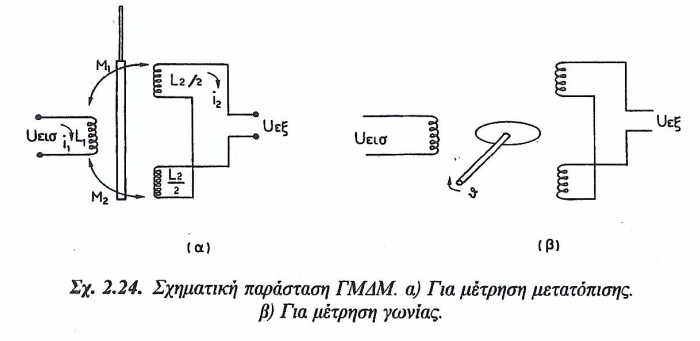
\includegraphics[width=\linewidth]{GMDM1.png}
    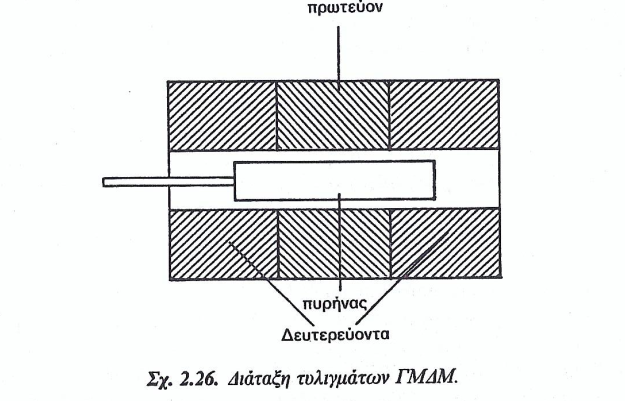
\includegraphics[width=\linewidth]{GMDM2.png}
\end{figure}
\emph{Σελ. 329-33}

\subsection{Περιγράψτε τη λειτουργία των οπτικών κωδικοποιητών μεταβολής}
Οι οπτικοί κωδικοποιητές μεταβολής αποτελούνται από ένα δίσκο ο οποίος αποτελείται από διαδοχικούς διαφανείς και αδιαφανείς τομείς. Πολλές φορές φέρουν δόντια, ώστε οι
προεξοχές να έχουν τον ρόλο του αδιαφανούς και οι εσοχές τον ρόλο του διαφανούς τομέα. 

Ο κωδικοποιητής προσαρμόζεται σε έναν άξονα και ακολουθεί την περιστροφή του. Από τη μια πλευρά του κωδικοποιητή υπάρχει μια πηγή φωτός και από την άλλη ένας δέκτης φωτός.
Καθώς περιστρέφεται ο δίσκος περιστρέφεται ο δίσκος εναλλάσονται οι διαφανείς και αδιαφανείς τομείς με αποτέλεσμα να παράγεται μια αλληλουχία παλμών το άθροισμα των οποίων 
δείχνει την γωνιακή θέση του άξονα. 

Η διακριτική ικανότητα ενός κωδικοποιητή εξαρτάται από τον αριθμό των παλμών (άρα των διαφανών και αδιαφανών τομέων του δίσκου). Πολλοί κωδικοποιητές χρησιμοποιούν 
και δεύτερο ζεύγος πομπού και δέκτη, δίνοντας παλμό για κάθε περιστροφή και τρίτο ζεύγος για προσδιορισμό της φοράς περιστροφής. 

Το μειονέκτημά τους είναι ότι δεν δείχνουν την απόλυτη θέση του άξονα, για αυτό απαιτούνται εξωτερικά κυκλώματα τα οποία μετρούν τους παλμούς και προσδιορίζουν τη θέση του
άξονα κάθε στιγμή.

\emph{Σελ. 333-4}


\section{Μέτρηση Ταχύτητας και Επιτάχυνσης}
\subsection{Περιγράψτε τη στροβοσκοπική μέθοδο μέτρησης περιστροφής ενός άξονα}
Ας υποθέσουμε ότι ένας άξονας περιστρέφεται με ταχύτητα περιστροφής $n\;r/sec$ και ότι μία λάμπα που φωτίζει τον άξονα αναβοσβήνει με συχνότητα $f$. Αν υπάρχει κάποιο 
σημάδι επάνω στον άξονα θα φαίνεται ακίνητο στην περίπτωση που $n=kf$, με $k$ ακέραιο. Η μέτρηση γίνεται μεταβάλλοντας την συχνότητα $f$ έως ότου κάποιο σημάδι του άξονα
που ορίζεται για αυτό το σκοπό φανεί ακίνητο. Συνήθως η συχνότητα κυμαίνεται από $2$ έως $400 Ηz$.

\emph{Σελ. 362-3}

\subsection{Περιγράψτε τη λειτουργία ταχογεννητριών}
Οι ταχογεννήτριες παράγουν μια τάση ανάλογη της ταχύτητας περιστροφής του άξονά τους.

\begin{itemize}
    \item Οι ταχογεννήτριες \textbf{εναλλασσόμενου} ρεύματος είναι κινητήρες κλωβού δύο τυλιγμάτων. Το ένα τύλιγμα τροφοδοτείται με με εναλλασσόμενο ρεύμα. Λόγω της 
        περιστροφής του άξονα επάγεται στο άλλο τύλιγμα μια εναλλασσόμενη τάση με πλάτος ανάλογο της ταχύτητας περιστροφής. Η συχνότητα είναι ίση με τη συχνότητα 
        τροφοδοσίας και η φάση $180^\circ$ ή $0^\circ$, ανάλογα με τη φορά περιστροφής του άξονα. Η ευαισθησία αυτών των ταχόμετρων είναι μερικά βολτ ανά $1000\; rpm$.
        Η συχνότητα της φάσης τροφοδοσίας είναι $50-60$ ή $400Hz$. 
    \item Η ταχογεννήτρια \textbf{συνεχούς} ρεύματος είναι μια συνηθισμένη γεννήτρια συνεχούς ρεύματος η οποία έχει κατασκευαστικά καλή ακρίβεια και ευαισθησία. Η
        τάση εξόδου της είναι ανάλογη της ταχύτητας περιστροφής του άξονα και η πολικότητά της αλλάζει όταν αλλάζει η φορά του άξονα. Χρησιμοποιείται για ταχύτητες
        μέχρι μερικές χιλιάδες $rpm$. Έχουν ευαισθησία αρκετά βολτ ανά $1000\; rpm$.
\end{itemize}

\emph{Σελ. 364-5}

\subsection{Εξηγήστε πότε ένας μετατροπέας ταχύτητας λέγεται σχετικός και πότε απόλυτος}

\begin{figure}[h!]
    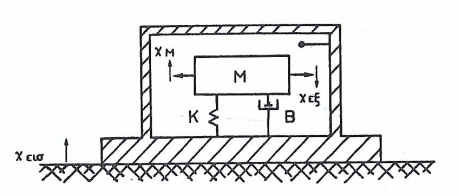
\includegraphics[width=\linewidth]{epitaxinsiometro.png}
    \caption{Βασικού τύπου επιταχυνσιόμετρο}
    \label{fig:5.1epitax}
\end{figure}

\begin{itemize}
    \item Ο \textbf{απόλυτος} μετατροπέας ταχύητας αποτελείται από ένα επιταχυνσιόμετρο (Σχ. \ref{fig:5.1epitax}) και έναν μετατροπέα θέσης.
        Γίνεται χρήση της  αδρανειακής δύναμης που ασκείται στη μάζα Μ του επιταχυνσιόμετρου για τη μέτρηση της ταχύτητας.
    \item \textbf{Σχετικός} λέγεται ο μετατροπέας ταχύτητας που μετρά τη σχετική ταχύτητα ενός τμήματος του μετατροπέα ως προς ένα άλλο.
\end{itemize}

\emph{Σελ. 369}

\subsection{Να υπολογίσετε τη συνάρτηση μεταφοράς ενός επιταχυνσιόμετρου βασικού τύπου (Σχ. 2)}
(Και πάλι δεν ξέρω κατά πόσο πιθανό είναι να πέσει αυτό σαν ερώτηση θεωρίας)

Έστω $x_{\epsilon\iota\sigma}$ η μετατόπιση του περιβλήματος, $x_{\epsilon\xi}$ η μετατόπιση της μάζας Μ ως προς το περίβλημα και $x_M$
η μετατόπιση της Μ ως προς το σύστημα αναφοράς. Οι δυνάμεις που επενεργούν πάνω στη Μ όταν υπάρξει κάποια κίνηση της επιφάνειας στήριξης 
είναι:

Η αντίδραση του ελατηρίου:

\begin{align*}
    F_1 = Kx_{\epsilon\xi}
\end{align*}

και η αντίδραση του αποσβεστήρα:

\begin{align*}
    F_2 = B\frac{dx_{\epsilon\xi}}{dt}
\end{align*}

Το άθροισμα των δυνάμεων προκαλεί επιτάχυνση στο σώμα:

\begin{align*}
    Kx_{\epsilon\xi} + B\frac{dx_{\epsilon\xi}}{dt} = M\frac{d^2x_M}{dt^2}
\end{align*}

Ισχύει, όμως, ότι: 

\begin{align*}
    x_M = x_{\epsilon\iota\sigma} - x_{\epsilon\xi} \Rightarrow Kx_{\epsilon\xi} + B\frac{dx_{\epsilon\xi}}{dt} = M*\left(\frac{d^2x_{\epsilon\iota\sigma}}{dt^2} - \frac{d^2x_{\epsilon\xi}}{dt^2}\right)
\end{align*}

Παίρνοντας τον μετασχηματισμό \foreignlanguage{english}{Laplace} προκύπτει η συνάρτηση μεταφοράς του συστήματος:

\begin{align*}
    \frac{X_{\epsilon\xi}}{X_{\epsilon\iota\sigma}} = \frac{s^2M}{s^2M + sB + K} &= \frac{s^2}{s^2 + s\frac{B}{M} + \frac{K}{m}} \\
    \intertext{Θέτοντας:} \\ 
    \omega_n = \sqrt{\frac{K}{M}} \\
    \zeta = \frac{B}{2\sqrt{KM}} \\
    \intertext{έχουμε:}
    \frac{X_{\epsilon\xi}}{X_{\epsilon\iota\sigma}} = \frac{1}{s^2 + 2s\zeta\omega_n + \omega^2}
\end{align*}

Όπου $\omega_n$ η κυκλική φασική συχνότητα και $\zeta$ ο συντελεστής απόσβεσης του συστήματος. Η $\omega_n$ είναι η συχνότητα που θα ταλαντωνόταν το σύστημα αν $Β=0$.

\emph{Σελ. 366-8}

\subsection{Να εξηγήστε γιατί το πιεζοηλεκτρικό επιταχυνσιόμετρο δεν μπορεί να μετρήσει σταθερή επιτάχυνση αφού υπολογίσετε την συνάρτηση μεταφοράς του}
Η μάζα $Μ$ πιέζει τον πιεζοηλεκτρικό κρύσταλλο ο οποίος συνήθως βρίσκεται σε τάση ακόμα και για μηδενική επιτάχυνση (Σχήμα \ref{piezoepitaxinsiometro}), έτσι ώστε ο μετατροπέας να μπορεί να 
μετρήσει επιταχύνσεις και προς τις δύο φορές. Αν θεωρήσουμε την έξοδο του πιεζοηλεκτρικού κρυστάλλου την τάση $\upsilon$ και σαν είσοδο την μεταβολή $x$ της διάστασης 
του κρυστάλλου κατά την διεύθυνση μέτρησης, η συνάρτηση μεταφοράς θα είναι:

\begin{align*}
    \frac{V(s)}{X(s)} = \frac{K_k\tau s}{1 + \tau s} 
    \intertext{$\tau$ μια χρονική σταθερά, $K_k$ η ευαισθησία} 
\end{align*}

Η μεταβολή $x$ που ορίσαμε εδώ είναι η μεταβολή $X_{\epsilon \xi}$ (η οποία ορίζεται σε μια πολύ προηγούμενη εξίσωση, βλέπε Πετρίδη), οπότε προκύπτει (συνδυάζοντας με μια
άλλη εξίσωση που ορίστηκε πάλι πιο πριν, ξαναβλέπε Πετρίδη):

\begin{align*}
    \frac{V(s)}{\gamma (s)}  = & \frac{K_k\tau s}{(1 + \tau s)(s^2 + 2s\zeta \omega_n + \omega_n^2)} \\
    \intertext{με περιοχή συχνοτήτων λειτουργίας: } \\
    &\ \ \frac{3}{\tau} < \omega < \frac{\omega_n}{5} 
\end{align*}

Από την περιοχή συχνοτήτων φαίνεται ότι το πιεζοηλεκτρικό επιταχυνσιόμετρο δεν μπορεί να λειτουργήσει ούτε σε πολύ χαμηλές ούτε σε πολύ υψηλές συχνότητες. Επειδή 
έχουν μεγάλη φυσική συχνότητα $\omega_n$, τα καθιστά κατάλληλα για μετρήσεις επιταχύνσεων που περιέχουν υψηλές αρμονικές, άρα απότομες μεταβολές της επιτάχυνσης, και άρα 
αδυνατούν στο να μετρήσουν σταθερή επιτάχυνση.

(Το γιατί τα πιεζοηλεκτρικά επιταχυνσιόμετρα δεν μπορούν να μετρήσουν σταθερή επιτάχυνση δεν το βρήκα στον Πετρίδη, οπότε κράτα μια επιφύλαξη για αυτό. Γιατί θεώρησε 
κάποιος ότι αυτή η ερώτηση ήταν καλή ιδέα δεν θα καταλάβω ποτέ)

\begin{figure}[h!]
    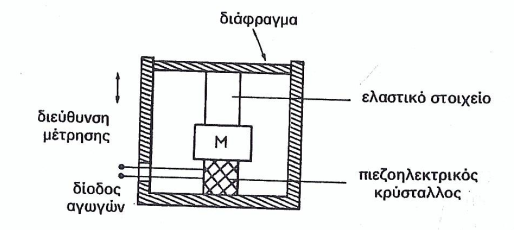
\includegraphics[width=\linewidth]{piezoepitaxinsiometro.png}
    \caption{Χαρακτηριστική κατασκευή πιεζοηλεκτρικού επιταχυνσιόμετρου}
    \label{piezoepitaxinsiometro}
\end{figure}

\emph{Σελ. 372-4}
\section{Μέτρηση Θερμοκρασίας}
\subsection{Να αναφέρετε και να εξηγήσετε πέντε βασικές ιδιότητες χρήσης θερμοζευγών}
\begin{itemize}
    \item Αν τα δύο υλικά του θερμοζεύγους είναι ομοιογενή, η θερμοηλεκτρεγερτική του δύναμη δεν εξαρτάται από την θερμοκρασία κανενός σημείου εκτός από τις θερμοκρασίες των ενώσεων 1
        και 2.
    \item Ας υποθέσουμε ότι η θερμοκρασία της ένωσης 1 είναι $Τ_1$ και της 2 είναι $Τ_2$, όπως στο σχήμα \ref{fig:7.1thermo1} και η θερμοηλεκτρεγερτική δύναμη είναι Ε. Έστω ότι καταστρέφεται η ένωση 1 και
        μεταξύ των υλικών Α και Β παρεμβάλλεται ένα άλλο υλικό Γ. Αν η θερμοκρασία των νέων ενώσεων ΒΓ και ΑΓ είναι $Τ_1$, τότε η θερμοηλεκτρεγερτική δύναμη θα είναι ίση με Ε ακόμα και αν
        η θερμοκρασία των τμημάτων του Γ έξω από τις ενώσεις ΑΓ και ΒΓ είναι διαφορετική από την $Τ_1$.
        \begin{figure}[h!]
            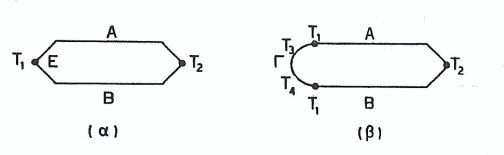
\includegraphics[width=\linewidth]{thermozevgi1.png}
            \caption{Θερμοστοιχείο με τρία υλικά και τρείς ενώσεις}
            \label{fig:7.1thermo1}
        \end{figure}
    \item Αν κοπεί ένα από τα δύο υλικά και παρεβληθεί ένα άλλο υλικό Γ, η ηλεκτρεγερτική δύναμη δεν μεταβάλλεται με την προϋπόθεση ότι οι ενώσεις π.χ. ΑΓ και ΓΑ έχουν την ίδια 
        θερμοκρασία $Τ_3$ ακόμη και αν η θερμοκρασία εκτός του Γ έξω από τις ενώσεις είναι διαφορετική από $Τ_3$.
        \begin{figure}[h!]
            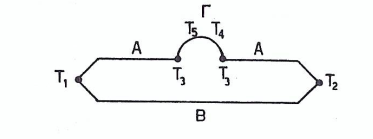
\includegraphics[width=\linewidth]{thermozevgi2.png}
            \caption{Θερμοστοιχείο με τρία υλικά και τέσσερεις ενώσεις}
            \label{fig:7.1thermo2}
        \end{figure}
    \item Έστω ένα θερμοζεύγος παράγει μια θερμοηλεκτρεγερτική δύναμη $Ε_1$ όταν οι θερμοκρασίες των ενώσεων 1 και 2 είναι $Τ_1$ και $Τ_2$ αντίστοιχα. Όταν οι θερμοκρασίες των ενώσεων
        1 και 2 είναι $Τ_2$ και $Τ_3$ αντίστοιχα, έστω η παραγόμενη θερμοηλεκτρεγερτική δύναμη είναι $Ε_2$. Αν οι θερμοκρασίες των ενώσεων 1 και 2 είναι $Τ_1$ και $Τ_3$ αντίστοιχα, η
        θερμοηλεκτρεγερτική δύναμη που θα παραχθεί θα είναι $Ε_1+Ε_2$.
    \item Αν η θερμοηλεκτρεγερτική δύναμη μεταξύ των υλικών Α και Γ είναι $Ε_{A\Gamma}$ και μεταξύ των υλικών Γ και Β είναι $Ε_{\Gamma B}$ η θερμοηλεκτρεγερτική δύναμη των
        υλικών Α και Β θα είναι $Ε_{A\Gamma} + E_{\Gamma B}$.
\end{itemize}

\emph{Σελ. 422-3}

\subsection{Να αναφέρετε δύο τρόπους σύνδεσης ενός θερμοστοιχείου με όργανο και να εξηγήσετε τη λειτουργία τους}
Για την μέτρηση της ηλεκτρεγερτικής δύναμης $Ε$ και την αντιστοίχησή της σε κάποια θερμοκρασία χρησιμοποιούνται όργανα μέτρησης τάσης. Τα όργανα αυτά είναι σε κάποια απόσταση από την ένωση
του θερμοζεύγους (Σχήμα \ref{thermozevgi3}). Για να μετρηθεί σωστά η $Ε$ με τις συνδέσεις των σχημάτων \ref{thermozevgi3}α και \ref{thermozevgi3}γ πρέπει οι ακροδέκτες του οργάνου να 
βρίσκονται στην ίδια θερμοκρασία. Για να μετρηθεί σωστά η $Ε$ με την σύνδεση \ref{thermozevgi3}β πρέπει οι ενώσεις 2 και 3 του θερμοζεύγους με τα καλώδια επέκτασης να 
βρίσκονται στην ίδια θερμοκρασία.  Στο σχήμα \ref{thermozevgi3}α η ένωση $2$ και στο σχήμα \ref{thermozevgi3}β οι ενώσεις $2$ και $3$ μπορούν να κρατηθούν σε σταθερές 
και επιθυμητές θερμοκρασίες με ένα μπάνιο (σήκω και κάνε ένα τώρα, ζέχνεις). Οι ενώσεις αυτές λέγονται 
ενώσεις αναφοράς και η θερμοκρασία τους θερμοκρασία αναφοράς. 

\begin{figure}[h!]
    \includegraphics[width=\linewidth]{thermozevgi3.png}
    \caption{Συνδέσεις θερμοστεοιχείου με όργανο}
    \label{thermozevgi3}
\end{figure}

(Ειλικρινά δεν είναι και η καλύτερη απάντηση αυτή αλλά \foreignlanguage{english}{I tried my best})

\emph{Σελ. 423-4}

\subsection{Περιγράψτε τους δύο τρόπους γραμμικοποίησης ενός θερμίστορ}
Τα θερμίστορ κατασκευάζονται από οξειδια μετάλλων και η αντίστασή τους μειώνεται καθώς η θερμοκρασία αυξάνει. 

Ένας τρόπος γραμμικοποίησης φαίνεται στο σχήμα \ref{thermistor}α. Οι τάσεις $V1$ και $V2$ εμφανίζουν γραμμική μεταβολή στο μέσον της περιοχής μέτρησης. Η $V1$ έχει 
θετική κλίση και η $V2$ αρνητική. Η διάταξη αυτή χρησιμοποιείται κυρίως σαν διαιρέτης τάσης που εξαρτάται από τη θερμοκρασία, δηλαδή η $V2$ εξαρτάται γραμμικά από 
τη θερμοκρασία. Η διάταξη στο σχήμα \ref{thermistor}β χρησιμοποείται σαν αντίσταση που μεταβάλλεται γραμμικά με τη θερμοκρασία.

(Πώς γίνεται μια ερώτηση θεωρίας να έχει ως απάντηση δύο σχήματα? Πιθανό αλλά μου φαίνεται λίγο περίεργο)

\begin{figure}[h!]
    \includegraphics[width=\linewidth]{thermistor.png}
    \caption{Δύο τρόποι γραμμικοποίησης ενός θερμίστορ}
    \label{thermistor}
\end{figure}

\emph{Σελ. 432}

\subsection{Τι γνωρίζετε για του ημιαγωγικούς μετατροπείς θερμοκρασίας;}
Οι πιο σημαντικοί ημιαγωγικοί μετατροπείς θερμοκρασίας είναι αντιστάσεις, δίοδοι και ολοκληρωμένα κυκλώματα.

\begin{itemize}
    \item Οι \textbf{ημιαγωγικές αντιστάσεις} έχουν θετικό συντελεστή θερμοκρασίας, συνήθως $0,8\%$ της πλήρους κλίμακας ανά $^{\circ}C$. Η γραμμικότητά τους είναι καλή.
        Οι τιμές των ημιαγωγικών αντιστάσεων σε κανονική θερμοκρασία ποικίλλει από δεκάδες $Ohm$ σε δεκάδες $K\Omega$. Μπορούν να χρησιμοποιηθούν σεσ γέφυρα όπως τα
        $RTD$ και τα θερμίστορ.
    \item Στις \textbf{διόδους} η μεταβολή της τάσης προς θερμοκρασία είναι $-2,3mV/^{\circ}C$ για ενώσεις πυριτίου και $-2,1mV/^{\circ}C$ για ενώσεις γερμανίου (όσο 
        αυξάνεται η θερμοκρασία μειώνεται η τάση). Η εξάρτηση της τάσης από τη θερμοκρασία σε διόδους και τρανζίστορ χρησιμοποιείται για κατασκευή μετατροπέων θερμότητας
        με γρήγορη απόκριση.
    \item Υπάρχουν \textbf{ολοκληρωμένα κυκλώματα} που λειτουργούν σαν πηγές ρεύματος των οποίων η ένταση εξαρτάται από τη θερμοκρασία. Χρησιμοποιούνται για γραμμικούς
        μετατροπείς θερμοκρασίας οι οποίοι είναι πολύ εύκολοι στη χρήση.
\end{itemize}

\emph{Σελ. 433}

\subsection{Ένα θερμοζεύγος (Σχήμα \ref{thermikozevgos})έχει τη μία ένωση σε $25^{\circ} C$ και την άλλη σε $Τ_1$. Αν η μετρούμενη τάση είναι $E_2=3,991mV$ 
ποιά είναι η τάση στο άκρο $T_1$?}
Μεταξύ $Τ_1$ και $Τ_2$ υπάρχει θερμοηλεκτρεργετική δύναμη $Ε_1 = 3,991 mV$. Αν θεωρήσουμε $T_3 = 0^{\circ}C$ μεταξύ $T_2$ και $T_3$ βλέπουμε από τον πίνακα 
\ref{82pinakas} ότι θα έχουμε $E_2 = 1,277mV$, αφού $T_2 - T_3 = 25^{\circ}C$. Άρα μεταξύ $T_1$ και $T_3$ θα έχουμε $E = E_1 + E_2 = 5,268mV$ (4η ιδιότητα 
θερμοζευγών, βλ. 8.1), άρα από τον πίνακα \ref{82pinakas} $T_1 = 100^{\circ}C$.

\begin{figure}[h!]
    \centering
    \begin{subfigure}[b]{0.4\linewidth}
        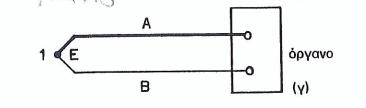
\includegraphics[width=\linewidth]{thermikozevgos.png}
        \caption{Σύνδεση θερμοστοιχείου με όργανο}
        \label{thermikozevgos}
    \end{subfigure}
    \begin{subfigure}[b]{0.4\linewidth}
        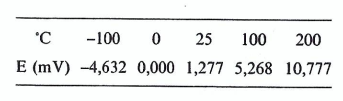
\includegraphics[width=\linewidth]{82pinakas.png}
        \caption{Πίνακας θερμοκρασιών}
        \label{82pinakas}
    \end{subfigure}
    \caption{}
\end{figure}

\emph{Ασκ. 2 Σελ. 434, τρόπος λύσης Σελ. 424}

\subsection{Η μεταβολή αντίστασης με τη θερμοκρασία ενός $RTD$ από λευκόχρυσο για την περιοχή $0-630^{\circ}C$ περιγράφεται από την εξίσωση $R_t=R_o(1+0.00398T - 0.588*10^{-6}T^2)$
όπου $R_t$ και  $R_o$ είναι οι αντιστάσεις του $RTD$ στις θερμοκρασίες $Τ$ και $0$ αντίστοιχα. Να υπολογισθεί το σφάλμα γραμμικότητας μέτρησης της θερμοκρασίας στις θερμοκρασίες 
$200^{\circ}C$ και $500^{\circ}C$.}

(Υποθετική λύση) Έστω ότι λείπει ο μη γραμμικός όρος $-0.588*10^{-6}T^2$. Τότε στους $200^{\circ}C$ θα είναι:

\begin{align*}
    & R_{200linear} = R_o(1+0.00398*200)=1.796R_o \\
    \text{eνώ }&R_{200real} = 1.75648R_o \text{ που είναι μια διαφορά } 2.224925\% \\
     \intertext{Ομοίως:} &\\
    &  R_{500linear} = 2.99R_o \\
    & R_{500real} = 2.843R_o \text{ που είναι μια διαφορά τάξης } 5.04029\% 
\end{align*} 

\emph{Ασκ. 9 Σελ. 435}

\section{Συστήματα προσαρμογής}
\subsection{Ένας μονοπολικός μετατροπέας έχει εύρος μετατροπής $0-25V$. Για έξοδο των $12\; bits$ να υπολογισθεί η διακριτική ικανότητα του μετατροπέα για την περίπτωση 
του δυαδικού κώδικα και του $BCD$.}
Για την περίπτωση του δυαδικού κώδικα αν ο μετατροπέας έχει $n\; bits$, η έξοδος μπορεί να πάρει $Ν=2^n$ διαφορετικές τιμές. Έτσι αν το εύρος μετατροπής είναι Ε, η διακριτική
ικανότητα του μετατροπέα θα είναι $E/2^n$. Στον κώδικα $BCD$ κάθε ψηφίο σε έναν δεκαδικό αριθμό παριστάνεται από $4\; bits$. Μετατροπείς που χρησιμοποιούν $BCD$ 
έχουν αριθμό $bits$ που έιναι πολλαπλάσιο του 4. Αν ο μετατροπέας $BCD$ έχει $4\; bits$, η έξοδος μπορεί να πάρει $N=10$ διαφορετικές τιμές ενώ αν έχει $8\; bits$ η
έξοδος μπορεί να πάρει $Ν=100$ διαφορετικές τιμές, άρα η διακριτική ικανότητα για $12\; bits$ θα είναι $\Delta E_{BCD}=\frac{2.5}{1000}$.

\emph{Σελ. 455-6}

\subsection{Ποιά τα πλεονεκτήματα μετάδοσης σήματος με ένταση ρεύματος $4-20mA$? Τι σημαίνει σφάλμα κλίμακας σε έναν $A/D$ μετατροπέα?}
Ας θεωρήσουμε για παράδειγμα ότι η έξοδος κάποιου μετατροπέα μεταβάλλεται από $0$ έως $10V$. Για να χρησιμοποιηθεί μετάδοση $4-20 mA$ πρέπει να γίνει μετατροπής της 
τάσης σε ρεύμα έτσι ώστε $0V$ να αντιστοιχούν σε $4 mA$ και $10V$ να αντιστοιχούν σε $20 mA$.Τα κύρια πλεονεκτήματα αυτού του τρόπου μετάδοσης είναι:

\begin{itemize}
    \item τα $4mA$ πασριστούν το μηδέν ενώ τα $0mA$ τη διακοπή του κυκλώματος
    \item η χρήση ρεύματος μειώνει την επίδραση των θορύβων
\end{itemize}

Το σφάλμα κλίμακας σημαίνει ότι η μέγιστη έξοδος δεν εμφανίζεται για την αντίστοιχη μέγιστη τιμή εισόδου. Με άλλα λόγια, η διαφορά της εισόδου κατά τη μεταβολή της 
εξόδου από $1110$ σε $1111$ με την είσοδο κατά τη μεταβολή της εξόδου από $0000$ σε $0001$ δεν ισούται με $E_{fs}-2LSB$. Το σφάλμα κλίμακας δίνεται σαν το ποσοστό 
της πλήρους κλίμακας.

\emph{Σελ. 453, 461}

\subsection{Για τη μετατροπή αναλογικού σήματος $7V$ χρησιμοποιείται ένας μετατροπέας $A/D$ κλιμακωτής ανόδου και ένας μετατροπέας $Α/D$ διαδοχικών προσεγγίσεων. Και οι δύο έχουν έξοδο 
$10\; bit$, $D/A$ με χρόνο μετατροπής $2\mu s$ και το εύρος μετατροπής τους είναι $0-12V$. Να υπολογισθεί ο χρόνος μετατροπής και των δύο μετατροπέων $A/D$ αν θεωρήσουμε ότι ο χρόνος
μετατροπής τους εξαρτάται μόνο από τον χρόνο μετατροπής του $D/A$}
    
\begin{itemize}
    \item Για την κλιμακωτή άνοδο έχουμε ότι $ΛΣΒ = \frac{12}{2^{10}} = 11.71875mV$ kai εφόσον η έξοδος του $D/A$ θα αυξάνει συνεχώς κατά την τιμή ενός $ΛΣΒ$ μέχρι να φτάσει τα $7V$, 
        θα έχουμε $x = |\frac{7000}{LSB}| = 598$ επαναλήψεις, άρα ο χρόνος μετατροπής θα είναι $598*2\mu s = 1.169ms$
    \item Η τεχνική των διαδοχικών προσεγγίσεων απαιτεί όσες μετατροπές όσα τα $bits$ στην έξοδο του $A/D$, άρα $x = n = 10$ kai $\Delta t = x * 2\mu s = 20\mu s$
\end{itemize}
\emph{Σελ. 462-3}

\subsection{Περιγράψτε την λειτουργία του μετατροπέα $A/D$ διπλής 
ολοκλήρωσης}
%\newpage

\begin{figure}[h!]
    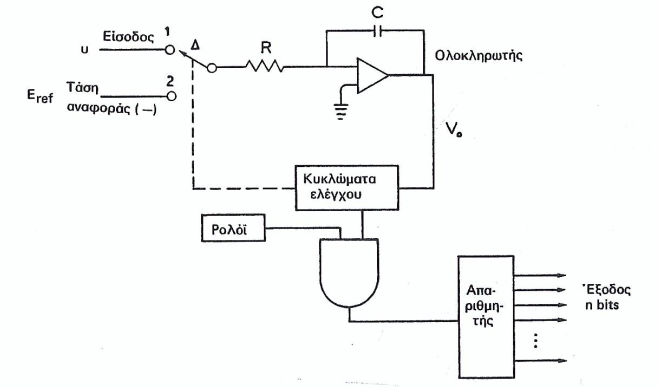
\includegraphics[width=\linewidth]{AD2olok.png}
    \caption{Μετατροπέας $A/D$ διπλής ολοκλήρωσης απλής μορφής}
\end{figure}
Μόλις δοθεί το ΣΕ ο διακόπτης Δ πηγαίνει στη θέση 1. Η ολοκλήρωση διαρκεί για ένα χρονικό διάστημα Τ το οποίο μετριέται στον απαριθμητή και αντιστοιχεί σε $Ν_1$. $Ν_1$ είναι το μέγιστο 
περιεχόμενο του απαριθμητή. Μετά την παρέλευση του χρονικού διαστήματος Τ η έξοδος του ολοκληρωτή είναι: 

\begin{align*}
    V_o=-\frac{1}{RC}\int^{T}_{0} \upsilon dt=-\frac{\upsilon}{RC}T
\end{align*}

Στη συνέχεια ο διακόπτης Δ πηγαίνει στη θέση 2 και ο απαριθμητής μηδενίζεται. Έτσι ο απαριθμητής αρχίζει να μετράει από το μηδέν ενώ η έξοδος του ολοκληρωτή μειώνεται γραμμικά δεδομένου
ότι η είσοδός του είναι η αρνητική τάση αναφοράς. Όταν μηδενισθεί η έξοδος του ολοκληρωτή τελειώνει η μετατροπή. Το περιεχόμενο $Ν_2$ του απαριθμητή έιναι η ψηφιακή παράσταση της 
αναλογικής εισόδου.Η έξοδος του ολοκληρωτή είναι: 

\begin{align*}
    V_o = -\frac{\upsilon}{RC}T + \frac{1}{RC} \int^t_0 E_{ref}dt = - \frac{\upsilon}{RC}T + \frac{E_{ref}}{RC}t
\end{align*}

Όταν $V_o = 0$, τότε $t=\frac{\upsilon}{E_{ref}}T$ και $N_2=\frac{\upsilon}{E_{ref}}N_1$.

Σε αυτόν τον μετατροπέα οι μεταβολές με το χρόνο ή την θερμοκρασία των $R$, $C$ και της συχνότητας του ρολογιού δεν παίζουν ρόλο (εκτός αν αλλάξουν κατά τη διάρκεια μιας μετατροπής).
Η γραμμικότητα αυτού του μετροπέα είναι πολύ καλή, αλλά ο χρόνος μετατροπής είναι πολύ μεγάλος.

\emph{Σελ. 464-5}

\subsection{Πρόκειται να σχεδιαστεί ένα σύστημα μετατροπής $A/D$ με εύρος μετατροπής $-10V$ εώς $10V$ και $10\;bits$ που μπορεί να μετατρέπει αναλογικά σήματα με μέγιστη ταχύτητα $5kHz$
και ταχύτητα δειγματοληψίας $100\; samples/sec$. Να υπολογισθεί ο απαιτούμενος χρόνος συγκράτησης του $S/H$ και ο χρόνος μετατροπής του μετατροπέα $A/D$}
\begin{align*}
    \Delta E = \frac{20}{2^{10}} = 19,53125*10^{-3}\;& \text{(δεν καταλαβαίνω γιατί αυτό είναι απαραίτητο)} \\
    \intertext{Χρόνος συγκράτησης:} \\
    \Delta t &= \frac{1}{2\pi5*10^3*2^{10}} \\ 
    \intertext{Χρόνος μετατροπής:}
    f_{conv} = \frac{100}{100^{-3}} &= 100kHz \Rightarrow \Delta t = \frac{1}{100*10^3} = 10^{-5}s
\end{align*}

\emph{Σελ. 467}

\subsection{Για έναν μονοπολικό μετατροπέα $A/D$ με $n\; bits$ και κύκλωμα συγκράτησης $S/H$ να υπολογίσετε τη μέγιστη συχνότητα που μπορεί να μετατρέψει χωρίς σφάλμα}
Έστω πλάτος σήματος $\text{E}_{FS}$. Αν $\Delta Ε$ το αναλογικό σήμα που αντιπροσωπεύει ένα $LSB$ μετατροπής, τότε η μέγιστη επιτρεπτή μεταβολή του σήματος προς μετατροπή είναι 
$\frac{\Delta \text{E}}{2}$. Αν το σήμα εισόδου είναι ημιτονοειδές με πλάτος $\text{Ε}_{FS}$ και φάση του είναι $2\pi ft$, ο μέγιστος ρυθμός μεταβολής εμφανίζεται για $t = 0$ και είναι $2\pi f E_{FS}$.
Τότε, $2 * 2 \pi fE_{FS} \leq \Delta E$. Αφού έχουμε μονοπολικό μετατροπέα, $\Delta E = \frac{E_{FS}}{2^n}$ άρα έχουμε ότι $f \leq \frac{1}{4\pi2^n\Delta t}$ όπου $\Delta t$ ο χρόνος
συγκράτησης του κυκλώματος $S/H$.


\emph{Σελ. 467}

\subsection{Να εξηγήσετε τη χρησιμότητα ενός κυκλώματος συγκράτησης $(S/H)$ και του πολυπλέκτη}
Κύκλωμα συγκράτησης: Για να γίνει σωστή η μετατροπή $A/D$, η αναλογική είσοδος δεν πρέπει να μεταβάλλεται πάνω από το όριο μεταβολής $1/2LSB$. Παρατηρούμε ότι κανονικά,
πολύ χαμηλές συχνότητες θα μπορούσαν να μετατραπούν από τους γρηγορότερους μετατροπείς. Για να ξεπερασθεί αυτό το πρόβλημα, η είσοδος πρέπει να κρατηθεί σταθερή. Για
αυτό το λόγο χρησιμοποιούνται τα κυκλώματα συγκράτησης, τα οποία κρατούν την έξοδό τους σταθερή (είσοδος του μετατροπέα) όταν λαβουν εντολή συγκράτησης. Υπάρχει, 
βέβαια χρόνος συγκράτησης, όμως είναι πολύ μικρός σε σχέση με το χρόνο μετατροπής, επτρέποντας την μετατροπή υψηλότερων συχνοτήτων.

Πολυπλέκτης: Έαν θέλουμε να μετατρέψουμε πολλά αναλογικά σήματα σε ψηφιακά, θα μπορούσαμε να χρησιμοποιήσουμε έναν μετατροπέα $A/D$ γαι κάθε σήμα. Όμως αυτή η λύση είναι
πολύ ακριβή, για αυτό έναν μετατροπέα $A/D$ μετά από έναν πολυπλέκτη. Η μετατροπή των σημάτων γίνεται διαδοχικά, με την προϋπόθεση ότι η ταχύτητα δειγματοληψίας που
απαιτείται για κάθε σήμα είναι τέτοια, ώστε να προλαβαίνει να ανταποκρίνεται ο μετατροπέας $A/D$.

Όταν έρθει η εντολή εκκίνησης στον πολυπλέκτη, η τιμή στην είσοδο των διευθύνσεων τη στιγμή εκείνη καθορίζει ποιά αναλογική είσοδος θα περάσει στην έξοδο, ενώ οι 
υπόλοιπες αναλογικές εισόδοι θα απομονωθούν.

\emph{Σελ. 467-8}

\subsection{Περιγράψτε την αρχή λειτουργίας ενός μετατροπέα $D/A$ ρεύματος}
Οι μετατροπείς $D/A$ ρεύματος λειτουργούν μέσω κυκλωμάτων που δημιουργούν ρεύματα $i$,$i/2$,$i/4$ κλπ. τα οποία αθροίζονται στην έξοδο (Σχήμα \ref{DArevmatos}). Αν μία δίοδος συνδεθεί σε λογικό 0, άγει και 
βραχυκυκλώνει το αντίστοιχο τρανζίστορ από το οποίο δεν περνάει ρεύμα. Αν μία δίοδος συνδεθεί σε λογικό 1, δεν άγει και το ρεύμα περνάει από το αντίστοιχο τρανζίστορ. Έτσι, το 
ρεύμα εξοδου εξαρτάται από την ψηφιακή είσοδο και η τιμή του καθορίζεται από τη σχέση (υποθέτουμε ότι η ψηφιακή λέξη είναι $8 bit$):

\begin{align*}
    I = K E_{ref} \left( b_7/2 + b_6/4 + b_5/8 + b_4/16 +b_3/32 + b_2/64 + b_1/128 + b_0/256 \right)
\end{align*}

\begin{figure}[h!]
    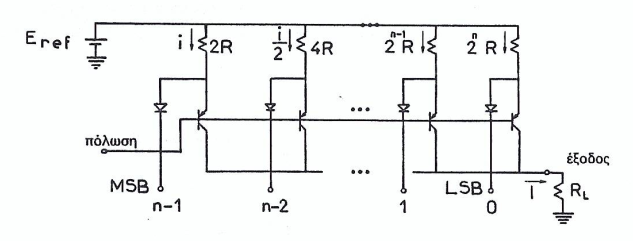
\includegraphics[width=\linewidth]{DArevma.png}
    \caption{Απλός μετατροπέας $D/A$ ρεύματος. Έχει πολλά μειονεκτήματα, όπως σημαντική εξάρτηση από θερμοκρασία, μεγάλη διαφορά στις τιμές των αντιστάσεων κλπ.}
    \label{DArevmatos}
\end{figure}

\emph{Σελ. 470-1}

\subsection{Να περιγραφεί η αρχή λειτουργίας ενός μετατροπέα $D/A$ τάσης}
Οι μετατροπείς $D/A$ μετατρέπουν ένα ψηφιακό σήμα σε αναλογικό συκγρίνοντας την αναλογική τάση που αντιπροσωπεύει το ψηφιακό σήμα με την τάση αναφοράς. Για ψηφιακή λέξη $8bit$ έχουμε
έξοδο: 

\begin{align*}
    \upsilon = K E_{ref} \left( b_7/2 + b_6/4 + b_5/8 + b_4/16 +b_3/32 + b_2/64 + b_1/128 + b_0/256 \right)
\end{align*}

Έστω ότι η είσοδος είναι Έστω ότι η είσοδος είναι 00000001. Ένα δυαδικό 1 συνδέει τον αντίστοιχο διακόπτη στη θέση 1 (δηλαδή στο αρνητικό άκρο της πηγής αναφοράς, Σχήμα \ref{DAtashs}). Έτσι
μόνο η 1η αντίσταση συνδέεται στην πηγή αναφοράς ενώ οι άλλες αντιστάσεις συνδέονται στη γη. Κατά συνέπεια η έξοδος θα είναι $\upsilon = -\frac{E_{ref}}{256R}R_o$. Αν η είσοδος είναι
00000011, $\upsilon = -3\frac{E_{ref}}{256R}R$.

\begin{figure}
    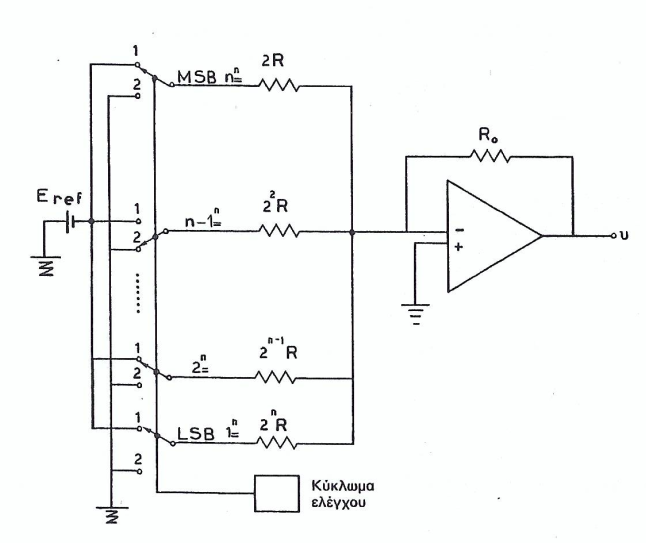
\includegraphics[width=\linewidth]{DAtashs.png}
    \caption{Μια απλή διάταξη μετατροπέα $D/A$ τάσης}
    \label{DAtashs}
\end{figure}

\emph{Σελ. 469-70}

\subsection{Τι είναι χρόνος αποκατάστασης σε έναν μετατροπέα $D/A$?}
Ο χρόνος που μεσολαβεί εώς ότου η έξοδος φτάσει την τελική τιμή με ακρίβεια $\pm1/2LSB$. Aυτόν τον χρόνο εννοούμε όταν λέμε χρόνος μετατροπής. Εξαρτάται από το είδος
των διακοπτών, το είδος των αντιστατών (αν έχουν αυτεπαγωγή ή όχι) και από τον ενισχυτή εξόδου (αν υπάρχει). Προδιαγράφεται για μια ορισμένη χωρητικότητα στην έξοδο.

\emph{Σελ. 473}

\end{document}
